\section{Filter design and implementation}\label{sec:filter}



\subsection{Block-parametric design}\label{sec:block}

\subsubsection{Block decomposition}\label{sec:bbbb}

We assume that medical devices produce 3D images with lateral dimensions that are integer multiples of some powers of two, like 128, 256, 512, etc.
Any cuboidal portion of image is completely determined by the Cartesian indices of its voxel of lowest and highest indices, and denoted as $Image([\ell_x, \ell_y, \ell_z],[h_x, h_y, h_z])$.

For the sake of simplicity, we assume a common size on the three image axes, and the corresponding image portion $B$, called \emph{block}, as a function of its element of the  lowest  block  coordinates $i,j,k\in\N$ and of block dimension $n$:
\[
B(i,j,k,n) := Image([in,jn,kn],[i(n+1),j(n+1),k(n+1)]) 
\]

\begin{figure}[htbp] %  figure placement: here, top, bottom, or page
   \centering
   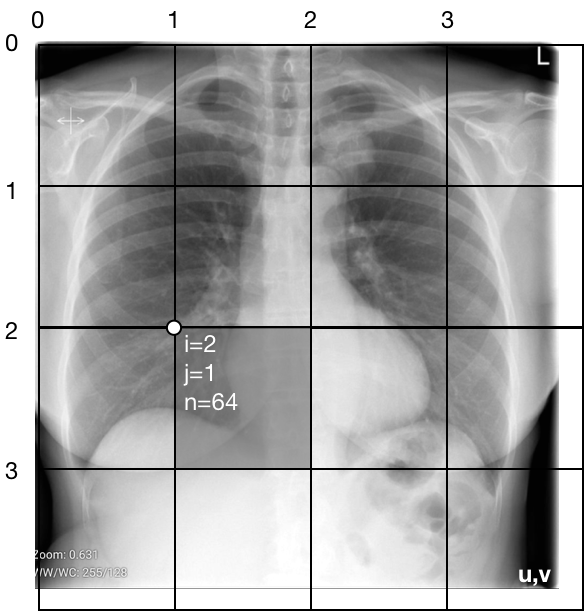
\includegraphics[width=2in]{figs/blocks} 
   \caption{A possible block partitioning of a radiologic image. The evidenced 2D block is $B([2,1,64]) = Image([128,64],[172,128)]$}
   \label{fig:blocks}
\end{figure}


Figure~\ref{fig:blocks} shows the block decomposition in a 2D case, with positive integer $u,v$ lateral sizes of image. Note that block sides do not necessarily correspond to image edges. 


\subsubsection{Block operator }\label{sec:bbbb}

\paragraph{Chain coordinates }\label{sec:bbbb} 
We are going to treat each image block independently from each other. Hence we map each image subspace $B(i,j,n)$ to the linear \emph{chain} space $C_2$ of dimension $n\times n$, using coordinate vectors $c_{h,k}\in \B^{n\times n} := \{0,1\}^{n\times n}$, where the basis element $c = c_{h,k} \in C_2$ is mapped via Cartesian-to-linear map to the Boolean vector 
\[
Image(h,k) \mapsto c_{h,k} := [0 \cdots 0\ 1\ 0 \cdots 0] \in \B^{n\times n}
\]
for each $0\leq h,k \leq n$, and where the (single) unit element is in position $nk + h \leq n\times n$.

Therefore, each pixel (or voxel) in a block image will be seen as a basis Boolean vector in $C_2$, and each subset of image elements, as the corresponding Boolean vector in $C_2$, with many ones as the cardinality of the subset.

\paragraph{Boundary operator }\label{sec:bbbb} For a fixed block size $n$, the boundary operator $\partial_d : C_d\to C_{d-1}$, with $d\in\{2,3\}$, will be constructed once and for all using the algorithm given in~\cite{}, and inlined in the generated boundary extraction code.

It is easy to see that the operator's matrix $[\partial_d]$ is \emph{very sparse}, since it contains $2\times d$ non-zero elements (ones) for each column (of length $n^d$), i.e.~4 ones and 6 ones for the 2D and 3D case, respectively. In fact the matrix of a linear operator between linear spaces contains by columns the basis element of the domain space, represented in the target space. In our case, the former is an image element (2-cube or 3-cube), represented as the chain of its boundary---i.e. either a 1-cycle of 4 edges, or  a 2-cycle of 6 faces, respectively.  

The number of rows of $[\partial_d]$ equates the dimension of the linear space $C_{d-1}$, i.e.~the number of $(d-1)$-cells---elementary $(d-1)$-chains---in the cellular partition of the image. To compute their number, we act in two steps. (a) First we map one-to-one the $n^d$ $d$-cells with $d$ adjacent $(d-1)$-cells, so getting $d\,n^d$ distinct basis elements of $C_{d-1}$. (b) Then we complete this bases by adjoining $n^{d-1}$ boundary elements for each of the $d$ dimensions of the image, so providing further $d\,n^{d-1}$ basis elements for $C_{d-1}$. The dimension of $C_{d-1}$, and therefore the number of rows of $[\partial_d]$ matrix is $d\,(n^{d-1}+n^{d}) = d\,n\,(1+n)^{d-1}$. The number of column equates the number of basis elements of $C_d$, i.e.~the number $n^d$ of block elements.

\paragraph{Sparsity and size of boundary matrix }\label{sec:bbbb} 

As we have seen, we have $2d$ non-zero elements for each column of $[\partial_d]$, so that their total number is $2d\,n^d$. The number of matrix element is $d\,n\,(1+n)^{d-1} \times n^d$, giving a ratio of 
\[
\frac{\mbox{non-zero\ elements}}{\mbox{total\ elements}} = 
\frac{2d\times n^d}{d\,n\,(1+n)^{d-1} \times n^d} =
\frac{2}{n+n^d}
\]
Using sparse matrices in CSC (Compressed Sparse Column) format we get a storage size:
\[
mem([\partial_d]_{n^d}) = 2\times \#\mbox{nzero} + \#\mbox{columns} = 2\times 2d\,n^d + n^d = (4d+1)n^d.
\]
In conclusion, for block size $n=64$, the matrix $[\partial_d]$ requires for 2D images $9\times 64^2=36,864$ memory elements, and for 3D images $13\times 64^3=3,407,872$ memory elements. Counting the bytes for the standard implementation of a sparse binary matrix (1 byte for values and 8 bytes for indices) we get $(18d+8)n^d$ bytes, giving $176$\,KB for 2D and $15.872$\,MB for 3D.

\subsubsection{Block boundary mapping}\label{sec:bbbb}

Here we refer directly to the 3D case.
Let us call \emph{segment} the bulk content $S$ of interest within the input 3D image of size $(u,v,w)$. We aim to compute the segment boundary $\partial_3 S$. 
First we set the size $n$ of the block, in order to decompose the input $Image(u,v,w)$ into a fair number 
\[
M = \ceil{u/n} \times \ceil{v/n} \times \ceil{w/n}
\] of blocks. 
Then we consider each image portion $c_{i,j,k} = S\cap B(i,j,k,n)$ and compute its (binary) coordinate representation  $[c]_{i,j,k}\in C_3(n,n,n)$. This one is a sparse binary vector of length $n^3$. Then assemble the $M$ representations $c$ of segment portions into a sparse binary matrix $\T{S}$, of dimension $n^d \times M$. Finally compute a matrix $\T{B}$ of boundary portions of $S$, represented by columns as chain coordinate vectors in $C_2$:
\[
\T{B} = [\partial_3(n,n,n)]\, \T{S}.
\]

Of course, the $\T{B}$ sparse matrix has the same column number $M$ of $\T{S}$, because each column contains the boundary representation of the corresponding $S\cap B_{i,j,k}$, and the number of rows of the operator, equal to the dimension of the linear space $C_2$.

\paragraph{Embedding}
A final computational step is needed, in order to embed the 2-chains in Euclidean space $\E^3$ and to assemble the whole resulting surface. In particular, we need to compute the \emph{embedding function} $\mu : C_0 \to \E^3$, where $C_0$ is the space of 0-chains, one-to-one corresponding to the vertices of the extracted surface. The simplest solution is to associate  four 0-cells to each 2-cell of the extracted surface, i.e.~to each non-zero entry in every column of \T{B}.  The $\mu$ function  can be computed by identifying, via  element position in the column, a triple of integer values $0\leq x\leq u, 0\leq y\leq v, 0\leq z\leq w$ for each vertex of the 2-cell.  The mapping can be implemented using a dictionary, thet will store the inverse coordinate transformation used at the beginning, i.e.~the one from linear to Cartesian coords, in order of not duplicating the output vertices.  

\paragraph{Assembling the surface portions}


\subsubsection{Block parallelism}\label{sec:bbbb}

\subsubsection{Reduced model}\label{sec:bbbb}







\subsection{Julia implementation}\label{sec:implementation}


\subsection{Code optimization}\label{sec:optimization}


\subsection{Performance analysis}\label{sec:analysis}

